% !TEX root = main.tex
\section{System Specifications}
\label{sec:specifications}
The proposed radio communication system switches between QPSK and QAM-16 modulation, at a fixed transmit power and bandwidth, in order to obtain adaptable sound quality.  The system use the 2.4GHz ISM band with a carrier frequency of 2.415GHz and 2.455GHz for the data path and BER path respectively. The system is designed for a transmission distance of 2 meter in an indoor environment.

Some key system specifications are listed in table \ref{tab:specs_data} and \ref{tab:specs_ber}. Table \ref{tab:specs_data} shows the parameters for the data path and the values are listed for low / high data rate transmission. Table \ref{tab:specs_ber} shows parameters for the simpler BER path. 
% !TEX root = main.tex
% Table generated by Excel2LaTeX from sheet 'specs'
\begin{table}[htbp]
  \centering
  \caption{System specifications - data path}
    \begin{tabular}{lc}
    \rowcolor[rgb]{ 0,  0,  0} \textcolor[rgb]{ 1,  1,  1}{\textbf{System Variables}}	& \textcolor[rgb]{ 1,  1,  1}{\textbf{Value}} 		\\
    \rowcolor[rgb]{ 0,  0,  0} \textcolor[rgb]{ 1,  1,  1}{} & \textcolor[rgb]{ 1,  1,  1}{\textbf{Low / High Data rate}} 				\\
    	Frequency $f_0$ 								& $\MainCarrierFreq$ MHz 							\\
    	Modulation 									& $\text{QPSK} / \text{QAM-64}$						\\
    	Bit per symbol $m$ 								& $2 /6$ 											\\
    	Sound sampling rate $f_s$  						& $11025 / 22050$ Hz 								\\
    	Bits per sound sample $b_s$ 						& $8 / 12$ bits 										\\
    	Sound datarate $R_{ss}$ 							& $\sourceDataRateQPSK / \sourceDataRateQAM$ kbits/s	\\
    	Channel coding 								& Hamming (4,7) 									\\

    \rowcolor[rgb]{ 0,  0,  0} \textcolor[rgb]{ 1,  1,  1}{\textbf{Packet Parameters}} & \textcolor[rgb]{ 1,  1,  1}{} 				\\
	Packet header size      							& $\headerBits $  bits								\\
    	Packet data length     							& $\packetDataSymbols$  symbols					 	\\
    	Packet size   									& $\packetDataBitsQPSK/ \packetDataBitsQAM$  bits		\\
    
    \rowcolor[rgb]{ 0,  0,  0} \textcolor[rgb]{ 1,  1,  1}{\textbf{Frame Parameters}} & \textcolor[rgb]{ 1,  1,  1}{} 				\\
    	Training sequence type 							& Barker										 	\\
    	Training sequence length							& $\barkerSymbols$ symbols 					 		\\
   	Training sequence size bits 						& $\barkerBitsQPSK / \barkerBitsQAM$ bits	 			\\
    	Frame size 									& $\frameSizeBitsQPSK / \frameSizeBitsQAM$ bits			\\
        
    \rowcolor[rgb]{ 0,  0,  0} \textcolor[rgb]{ 1,  1,  1}{\textbf{Burst Parameters}} & \textcolor[rgb]{ 1,  1,  1}{} 					\\
    	Guard period 									& $\guardSymbols$ symbols							\\
    	Burst size 										& $\burstSizeBitsQPSK / \burstSizeBitsQAM$ bits 			\\
    	
    \rowcolor[rgb]{ 0,  0,  0} \textcolor[rgb]{ 1,  1,  1}{\textbf{Transmission Characteristics}} & \textcolor[rgb]{ 1,  1,  1}{} 		\\
    	System bit rate $R_b$ 							& $191,35 / 577,18$ kbits/s 							\\
    	Symbol rate $R_s$ 								& $95,67 / 96,20$ ksymbols/s 							\\
    	Pulse shaping filter 								& root raised cosine 									\\
    	Pulse shaping filter parameter $\alpha$ 				& $0.3$ 											\\
    	Minimum signal bandwidth $\Delta f$ 				& $62,2 / 62,5$ kHz 									\\
    \end{tabular}
  \label{tab:specs_data}
\end{table}

\begin{table}[htbp]
  \centering
  \caption{System specifications - ber path}
    \begin{tabular}{lc}
    \rowcolor[rgb]{ 0,  0,  0} \textcolor[rgb]{ 1,  1,  1}{\textbf{System Variables}}	& \textcolor[rgb]{ 1,  1,  1}{\textbf{Value}} 		\\
    \rowcolor[rgb]{ 0,  0,  0} \textcolor[rgb]{ 1,  1,  1}{} & \textcolor[rgb]{ 1,  1,  1}{\textbf{Low / High Data rate}} 				\\
    	Frequency $f_0$ 								& $\BERCarrierFreq$ MHz 							\\
    	Modulation 									& $\text{QPSK}$									\\
	
    \rowcolor[rgb]{ 0,  0,  0} \textcolor[rgb]{ 1,  1,  1}{\textbf{Packet Parameters}} & \textcolor[rgb]{ 1,  1,  1}{} 				\\
	Packet header size      							& $\headerBits $  bits								\\
    	Packet size									& $\BERDataBits$  bits					 			\\
    
    \rowcolor[rgb]{ 0,  0,  0} \textcolor[rgb]{ 1,  1,  1}{\textbf{Frame Parameters}} & \textcolor[rgb]{ 1,  1,  1}{} 				\\
    	Training sequence type 							& Barker										 	\\
    	Training sequence length							& $\barkerSymbols$ symbols 					 		\\
   	Training sequence size bits 						& $\barkerBitsQPSK$ bits	 							\\
    	Frame size 									& $\BERFrameSize$ bits								\\
    	
    \rowcolor[rgb]{ 0,  0,  0} \textcolor[rgb]{ 1,  1,  1}{\textbf{Transmission Characteristics}} & \textcolor[rgb]{ 1,  1,  1}{} 		\\
    	System bit rate $R_b$ 							& $\BERDataRate$ kbits/s 							\\
    	Symbol rate $R_s$ 								& $\BERSymbolRate$ ksymbols/s 						\\
    	Pulse shaping filter 								& root raised cosine 									\\
    	Pulse shaping filter parameter $\alpha$ 				& 0.3 											\\
    	Minimum signal bandwidth $\Delta f$ 				& $62,2 / 62,5$ kHz 									\\
    \end{tabular}
  \label{tab:specs_ber}
\end{table}


The burst format for the transmitted data is shown in figure \ref{fig:burst_format}. The bursts are different when using QPSK and QAM-16 modulation, because the same number of training symbols maps to a different number of bits. The data packages (a and b) is transmitted continuously with the indicated guard period. The BER packages is very small compared to the data packages, and is only transmitted ones per received data package. Thus no guard period is specified for these packages. 
% !TEX root = main.tex
\begin{figure} 
    \centering
  \subfloat[QPSK data package\label{1a}]{%
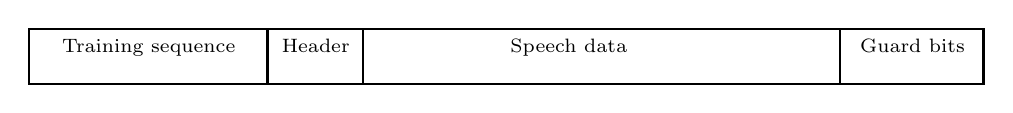
\begin{tikzpicture}[                
                    slot/.style={
            		text centered,
			font=\scriptsize,
			align=center,
			anchor=center,
			minimum height=0.7cm
            	}]
\draw[thick] (0,0) rectangle (\linewidth, -0.7);
\draw[thick] (0.25\linewidth,0) -- ++(0, -0.7);
\draw[thick] (0.35\linewidth,0) -- ++(0, -0.7);
\draw[thick] (0.85\linewidth,0) -- ++(0, -0.7);

\draw
(0,0) node[slot, minimum width=0.25\linewidth, anchor=north west](barker){Training sequence \\ \barkerBitsQPSK}
(0.25\linewidth,0)  node[slot, minimum width=0.1\linewidth, anchor=north west](barker){Header \\ \headerBits}
(0.35\linewidth,0) node[slot, minimum width=0.43\linewidth, anchor=north west](barker){Speech data \\ \packetDataBitsQPSK}
(0.85\linewidth,0) node[slot, minimum width=0.15\linewidth, anchor=north west](barker){Guard bits \\ \guardBitsQPSK}
;	

\end{tikzpicture}
}
  \\
  \subfloat[QAM-64 data package\label{1b}]{%
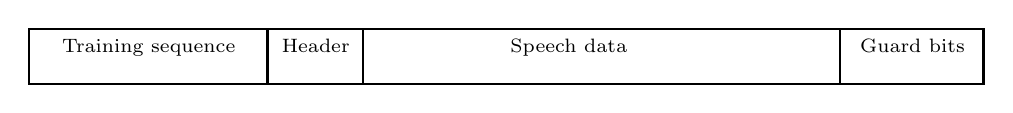
\begin{tikzpicture}[                
                    slot/.style={
            		text centered,
			font=\scriptsize,
			align=center,
			anchor=center,
			minimum height=0.7cm
            	}]
\draw[thick] (0,0) rectangle (\linewidth, -0.7);
\draw[thick] (0.25\linewidth,0) -- ++(0, -0.7);
\draw[thick] (0.35\linewidth,0) -- ++(0, -0.7);
\draw[thick] (0.85\linewidth,0) -- ++(0, -0.7);

\draw
(0,0) node[slot, minimum width=0.25\linewidth, anchor=north west](barker){Training sequence \\ \barkerBitsQAM}
(0.25\linewidth,0)  node[slot, minimum width=0.1\linewidth, anchor=north west](barker){Header \\ \headerBits}
(0.35\linewidth,0) node[slot, minimum width=0.43\linewidth, anchor=north west](barker){Speech data \\ \packetDataBitsQAM}
(0.85\linewidth,0) node[slot, minimum width=0.15\linewidth, anchor=north west](barker){Guard bits \\ \guardBitsQAM}
;	

\end{tikzpicture}}
\\
  \subfloat[QPSK BER package\label{1c}]{%
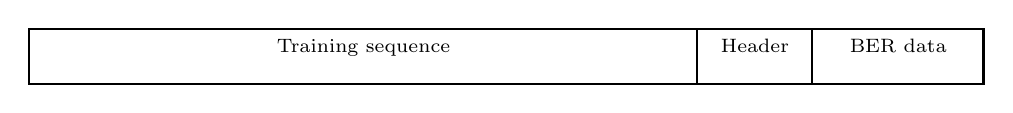
\begin{tikzpicture}[                
                    slot/.style={
            		text centered,
			font=\scriptsize,
			align=center,
			anchor=center,
			minimum height=0.7cm
            	}]
\draw[thick] (0,0) rectangle (\linewidth, -0.7);
\draw[thick] (0.70\linewidth,0) -- ++(0, -0.7);
\draw[thick] (0.82\linewidth,0) -- ++(0, -0.7);

\draw
(0,0) node[slot, minimum width=0.7\linewidth, anchor=north west](barker){Training sequence \\ \barkerBitsQPSK}
(0.70\linewidth,0)  node[slot, minimum width=0.12\linewidth, anchor=north west](barker){Header \\ \headerBits}
(0.82\linewidth,0) node[slot, minimum width=0.18\linewidth, anchor=north west](barker){BER data \\ \BERDataBits}
;	

\end{tikzpicture}}
  \caption{Burst format for QPSK(a) and QAM-64(b) modulated data bursts, and QPSK modulated BER burst (c)}
  \label{fig:burst_format} 
\end{figure}
 